\chapter*{Introduction}
\addcontentsline{toc}{chapter}{Introduction}

Le traitement du sujet faisant l'objet de cette étude a trait au domaine des ressources humaines dans le cadre du fonctionnement d'une entreprise où se côtoient différents groupes humains  et catégories de salariés dans diverses fonctions.\\
La gestion des ressources humaines a évolué et a développé des méthodes et des règles qui tiennent compte du contexte et des impératifs amenant à chaque fois les responsables à opter pour la méthode la plus appropriée tant au niveau organisationnel qu'en termes de coût pour en rentabiliser tous ses aspects.\\
Cette approche des décideurs est en réalité dictée par l'importance du contexte d'évolution de toute entreprise quelle que soit son activité et le degré d'impact de  chaque méthode d'évaluation de ces ressources humaines.\\

 
Aujourd'hui, les entreprises évoluent dans un environnement de plus en plus concurrentiel, changeant et complexe. En particulier, sur le marché de l'emploi où règne une concurrence exacerbée, l'exigence première est non seulement de recruter des ressources humaines de qualité, présentant un haut niveau de qualification, mais aussi de les fidéliser « réduire les comportements d'absentéisme et de démission » ainsi que de les motiver « des employés plus efficaces et plus appliqués ».\\
L'investissement sur les collaborateurs a un impact direct sur la satisfaction client, et réciproquement.\\
Le lien entre la satisfaction des employés et celle des clients est indiscutable. Des employés heureux ne signifient pas uniquement que ces employés ont le moral mais qu'ils seront plus efficaces et plus appliqués.\\ 
Selon une récente étude de Gallup, le désengagement des employés coûte plus de 300 milliards de \$US par an à l'industrie américaine. \\
Une autre étude montre que 72\% des employés motivés sont persuadés qu'ils peuvent influencer positivement le service clients. Cette étude visait à déterminer l'impact des employés motivés sur la satisfaction des clients :
\begin{itemize}
\item	Premièrement, le niveau d'engagement des employés a un impact sur la satisfaction des services fournis aux clients. A chaque augmentation de deux points de la motivation de l'employé, la satisfaction du client augmente d'un point.
\item	Deuxièmement, globalement environ 20\% des variations sur le score de satisfaction sont liées aux changements de scores des employés.\\
\end{itemize}

La motivation et satisfaction des employés sont fluctuantes et varient en fonction de très nombreux facteurs. En entreprise, il est question de bien-être et de volonté et pour que les salariés restent satisfaits et motivés, l’entreprise doit rester attentive à leurs besoins, au regard bien sûr de leur mérite\\
Ces besoins sont schématisés par la pyramide des besoins, une théorie élaborée à partir des observations réalisées dans les années 1940 par le psychologue Abraham Maslow sur la motivation. 

%inclusion d'une mage dans le document
\begin{figure}[!ht]
\begin{center}
%taille de l'image en largeur
%remplacer "width" par "height" pour régler la hauteur
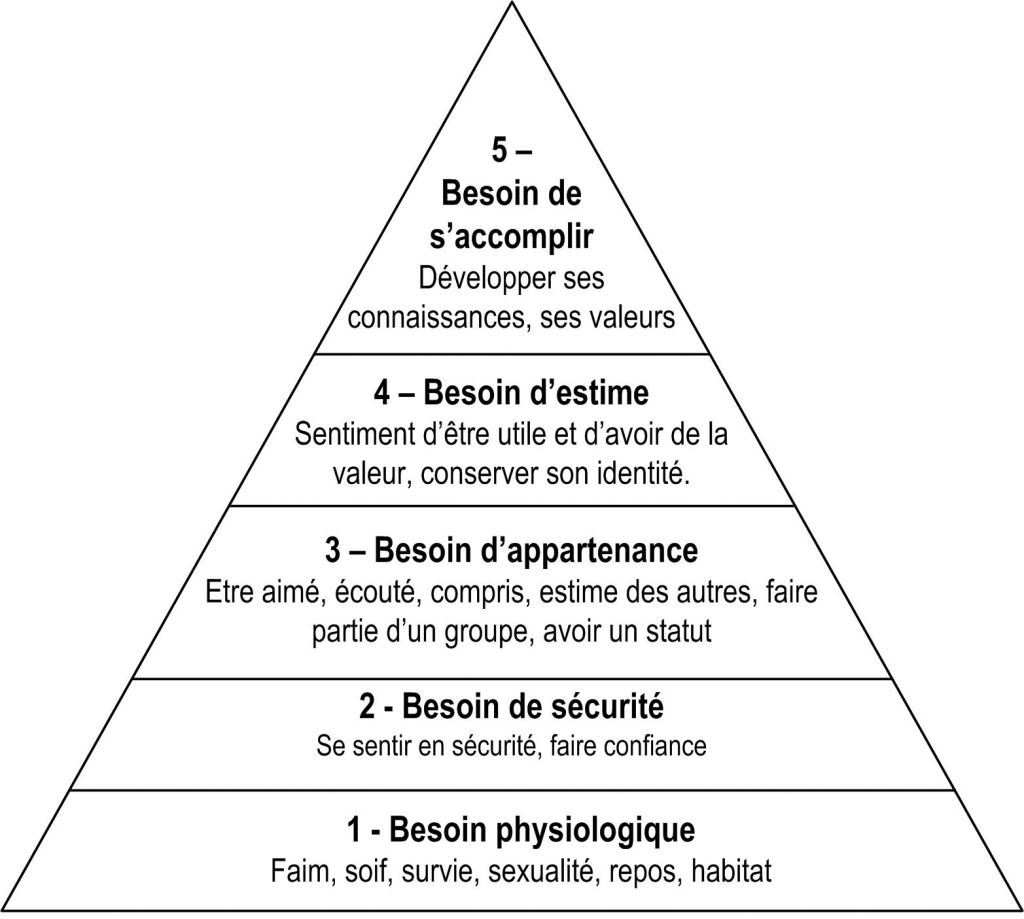
\includegraphics[width=9cm]{introduction/schema_introduction}
\end{center}
%légende de l'image
\caption{pyramide des besoins}
\end{figure}

\newpage

Voici quelques pistes utilisées par les entreprises aujourd’hui pour entretenir la motivation et satisfaction des salariés :
\begin{enumerate}
\item la motivation par le cadre de travail
\item la motivation par les avantages
\item la motivation par un voyage
\item La motivation par l’argent \\
\end{enumerate}

La promotion et/ou prime  peuvent être accordées en fonction des objectifs atteints par le salarié, ou en fonction du nombre d'années passées dans l'entreprise, une clause du contrat de travail prévoit fréquemment l'accord automatique de ces avancements, et suite à une simple demande de votre part, votre employeur appréciera alors vos résultats et vos compétences pouvant justifier une augmentation de vos responsabilités.\\
En plus de vos capacités techniques et intellectuelles, il peut être très avantageux de faire preuve de fiabilité et d'empathie.\\ Le contact relationnel avec les supérieurs et collègues peut s'avérer déterminant lorsqu'il s'agit d'arbitrer l'attribution d'une promotion.\\

Il existe 3 manières de promouvoir les employés :
\begin{enumerate}
\item Promouvoir les plus compétents
\item Promouvoir les moins compétents
\item Promouvoir au hasard
\end{enumerate}
\newpage
D’après le principe de Peter qui part du postulat que : «  tout employé compétent sera promu tôt ou tard à un poste qui surpasse ses compétences »,avec comme conséquence à terme d'avoir tous les postes occupés par des incompétents (situation inimaginable dans la pratique).
La solution qui est proposée pour un dirigeant constatant qu'il a des cadres supérieurs incompétents, c’est de recourir à la « sublimation percutante » consistant à accorder à une personne incompétente une promotion vers un poste plus prestigieux en apparence, mais en fait à responsabilité très inférieure, et pour les personnes constatant leur propre incompétence c’est de se maintenir à un poste auquel on est compétent.Ceci , non seulement dans l'intérêt de l'organisation où l'on travaille, mais aussi parce qu'être compétent à son poste est un facteur de bonheur personnel. Toutefois, Peter constate que le refus d'une promotion est mal vu par l'entourage des personnes..\\
Des chercheurs italiens ont réussi à prouver de manière scientifique que la meilleure manière d'attribuer les promotions c’était de les distribuer au hasard. Mais aussi rigoureuse soit-elle, cette expérience devrait ne servir à rien.\\
Pour faire cette recherche, ils sont partis de leur envie de contrer le "Principe de Peter", ils se sont lancés à la recherche d’un moyen de distribuer les promotions. Ils ont mis au point un simulateur qui compare les performances de l’entreprise selon trois scénarios. Dans le premier, la société promeut les employés les plus compétents. Dans le deuxième, elle choisit au contraire les moins compétents. Dans le dernier, elle nomme les managers au hasard. Et là, les chercheurs découvrent qu'avec la méthode aléatoire, la productivité augmente d’une dizaine de points! Alors qu’avec les deux autres scénarios, elle baisse, inévitablement.\\
 Observation: Les chercheurs soulignent néanmoins que la promotion au mérite n’est pas nécessairement plus juste. La mesure du mérite par un manager comporte une part de subjectivisme. Il reste que la promotion au hasard, même si son efficacité est prouvée, est indéfendable vis-à-vis des équipes. Et donc se pose la question de savoir comment motiver ses salariés si leur implication n’est pas récompensée?\\
Ce qui nous amène à mon travail car pour garder la motivation et en même temps avoir des résultats moins subjectifs , nous nous  proposons d’appliquer la méthode au mérite c’est-à-dire attribuer les promotions aux plus compétents en introduisant la solution informatisée en minimisant l’impact humain au maximum.\\   


\section*{Problématique}

L’un des coûts les plus élevé des entreprises est le roulement du personnel.  Un des plus grand défis est certainement de trouver le moyen de créer un environnement favorisant la mobilisation qui peut engendrer la productivité.\\
Non seulement, il est coûteux de procéder à des modifications d'organigramme (mouvement du personnel,mais les changements apportés affectent aussi le moral du reste du personnel. Afin de minimiser cela, l’entreprise doit s’employer à satisfaire et motiver ses salariés « primes, promotions, … », mais la répartition des promotions entre plusieurs individus exerçant la même fonction dans une même unité de production est un éternel sujet de discussions. Comment faut-il augmenter les salariés? Faut-il attribuer une promotion à tel salarié mais pas à l’autre ? Quelle prime donner à qui ? Et surtout comment attribuer ces primes de manière juste et équitable envers tous les employés ? Car la mesure du mérite par un manager comporte un aspect  subjectif.\\


\section*{Objectif}
Une solution qui peut paraître simple consiste à construire un outil d’aide à la décision pour le classement des salariés sur la base du mérite et de manière décroissante .Cela n’écartera toujours pas l’impact humain mais le minimisera car l’outil a pour but principal de guider les managers dans leurs décisions et de rassurer les employés par rapport à l’équité de la décision.\\
 \\
L’objectif de mon projet est de concevoir un outil d’aide à la décision pour apporter des réponses pertinentes à la problématique d’attribution de promotion ou de prime et cela en testant différentes méthodes d’évaluation des salariés d’une entreprise.  


\newpage




